\documentclass[11pt]{article}
\usepackage{coling2014}
\usepackage{times}
\usepackage{url}
\usepackage{latexsym}
\usepackage{graphicx}

%\setlength\titlebox{5cm}

% You can expand the titlebox if you need extra space
% to show all the authors. Please do not make the titlebox
% smaller than 5cm (the original size); we will check this
% in the camera-ready version and ask you to change it back.


\title{Modelling of Adjectives in the Ontology-Lexicon Interface}

\author{John P. M\textsuperscript{c}Crae \\
  Affiliation / Address line 1 \\
  Affiliation / Address line 2 \\
  Affiliation / Address line 3 \\
  {\tt email@domain} \\\And
  Francesca Quattri, Chrisitina Unger, Philipp Cimiano \\
  Affiliation / Address line 1 \\
  Affiliation / Address line 2 \\
  Affiliation / Address line 3 \\
  {\tt email@domain} \\}

\date{}

\begin{document}
\maketitle
\begin{abstract}
The ontology-lexicon interface has become an important and successful tool for handling problems in NLP (cite, cite, cite). The foundation of these models based on a separation of the ontological and lexical layers by means of the principle of semantics by reference to an ontology in description logics. However, as noted by other authors, the use of first order logic (hence also description logics) is while effective for nouns and verbs breaks down in the case of adjectives. We propose that this is primarily due to a lack of logical expressivity in the ontology. In particular, many adjectives are i) gradable requiring fuzzy or non-monotonic semantics or ii) operator adjectives require second-order logic. We consider  how we can handle the ontology-lexicon interface in the face of these more complex logical formalism, and show how these can be backward engineered into OWL based modelism by means of pseudo-classes, with application to question answering.
\end{abstract}

\section{Introduction}
\label{intro}

%
% The following footnote without marker is needed for the camera-ready
% version of the paper.
% Comment out the instructions (first text) and uncomment the 8 lines
% under "final paper" for your variant of English.
% 
\blfootnote{
    %
    % for review submission
    %
    \hspace{-0.65cm}  % space normally used by the marker
    Place licence statement here for the camera-ready version, see
    Section~\ref{licence} of the instructions for preparing a
    manuscript.
    %
    % % final paper: en-uk version (to license, a licence)
    %
    % \hspace{-0.65cm}  % space normally used by the marker
    % This work is licensed under a Creative Commons 
    % Attribution 4.0 International Licence.
    % Page numbers and proceedings footer are added by
    % the organisers.
    % Licence details:
    % \url{http://creativecommons.org/licenses/by/4.0/}
    % 
    % % final paper: en-us version (to licence, a license)
    %
    % \hspace{-0.65cm}  % space normally used by the marker
    % This work is licenced under a Creative Commons 
    % Attribution 4.0 International License.
    % Page numbers and proceedings footer are added by
    % the organizers.
    % License details:
    % \url{http://creativecommons.org/licenses/by/4.0/}
}

\begin{figure*}
    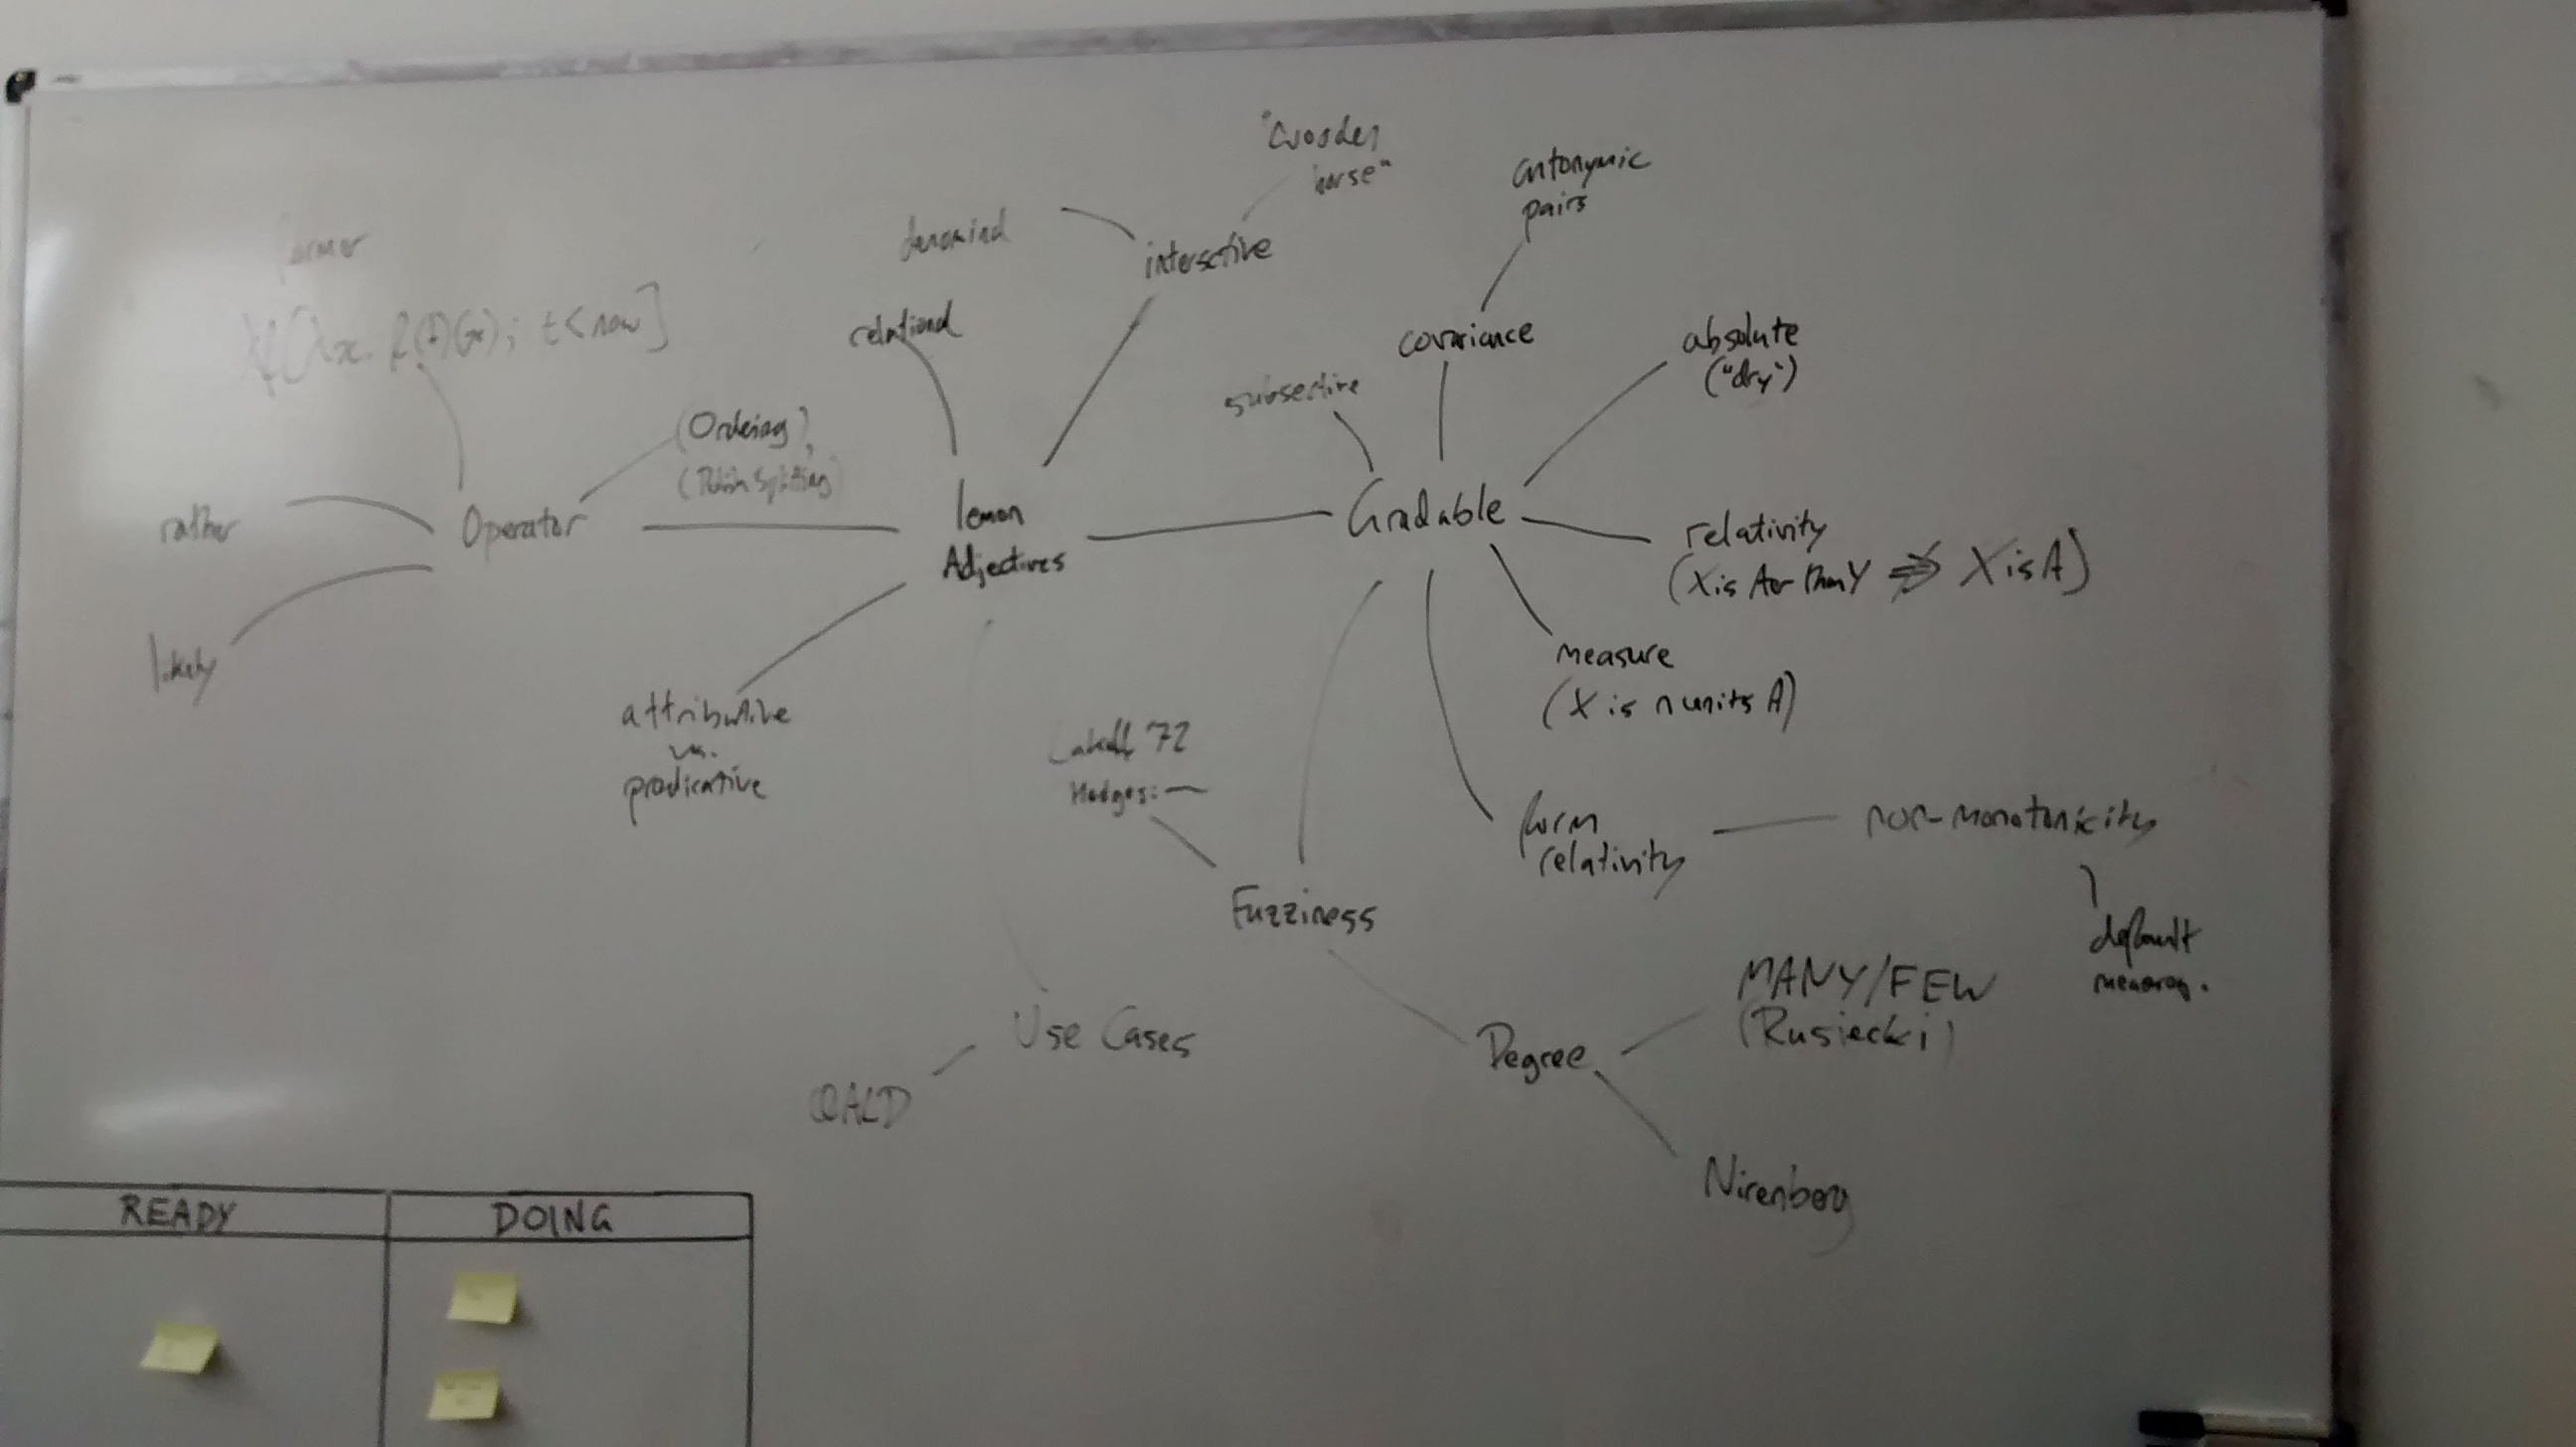
\includegraphics[width=\textwidth]{mindmap.jpg}
\end{figure*}

\section*{Acknowledgements}

\bibliographystyle{acl}
\bibliography{cogalex-adjectives}

\end{document}
